73. \begin{figure}[ht!]
\center{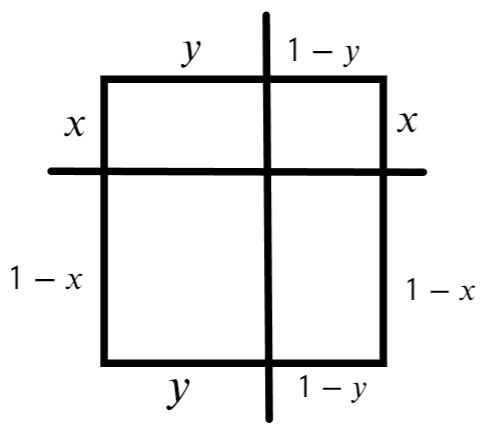
\includegraphics[scale=0.35]{issl9-73.png}}
\end{figure}\\
Обозначим сторону левого верхнего прямоугольника буквами $x$ и $y.$ Тогда произведение площадей равно $xy(1-x)(1-y)=(x-x^2)(y-y^2).$ График квадратичной функции $x-x^2$ представляет из себя параболу, ветви которой направлены вниз, а значит максимальное значение достигается в вершине, то есть при $x=-\cfrac{-1}{-2}=\cfrac{1}{2}.$ Оно равно $\cfrac{1}{2}-\cfrac{1}{4}=\cfrac{1}{4}.$ Второй множитель --- такая же функция, поэтому $S\leqslant \cfrac{1}{4}\cdot \cfrac{1}{4}=\cfrac{1}{16},$ ч.т.д.\\
